\documentclass[11pt,a4paper]{article}

\usepackage[margin=1in]{geometry}
\usepackage[T1]{fontenc}
\usepackage{lmodern}
\usepackage{microtype}
\usepackage{amsmath,amssymb,amsthm}
\usepackage{mathtools}
\usepackage{booktabs}
\usepackage{enumitem}
\usepackage{xcolor}
\usepackage[hidelinks]{hyperref}
\usepackage{tikz}
\usetikzlibrary{arrows.meta,positioning,calc,decorations.pathreplacing}

% Theorem environments
\newtheorem{theorem}{Theorem}[section]
\newtheorem{proposition}[theorem]{Proposition}
\newtheorem{lemma}[theorem]{Lemma}
\newtheorem{corollary}[theorem]{Corollary}
\newtheorem{definition}[theorem]{Definition}
\newtheorem{remark}[theorem]{Remark}

% Notation
\newcommand{\phig}{\varphi}
\newcommand{\Jcost}{J}
\newcommand{\Ecoh}{E_{\mathrm{coh}}}
\newcommand{\muStar}{\mu_{\star}}
\newcommand{\RS}{Recognition Science}
\newcommand{\SM}{Standard Model}
\newcommand{\Epass}{E_{\mathrm{passive}}}

% Claim tags
\newcommand{\PROVED}{\textcolor{blue!70!black}{\footnotesize\textsf{[PROVED]}}}
\newcommand{\HYP}{\textcolor{orange!80!black}{\footnotesize\textsf{[HYP]}}}
\newcommand{\CERT}{\textcolor{teal}{\footnotesize\textsf{[CERT]}}}
\newcommand{\VAL}{\textcolor{purple!70!black}{\footnotesize\textsf{[VAL]}}}

\title{\textbf{Why Three Generations?\\
The Geometric Origin of Generation Torsion $\{0,11,17\}$\\
from Cube Combinatorics in $D=3$}\\[0.5em]
\large Paper VI: Generation Structure}
\author{Jonathan Washburn\\
\small Recognition Science Research Institute, Austin, Texas\\
\small \texttt{washburn.jonathan@gmail.com}}
\date{\today}

\begin{document}
\maketitle

\begin{abstract}
The Standard Model contains three generations of fermions but offers no
explanation for this count nor for the specific mass ratios between
generations.  This paper derives the generation torsion
$\tau_g\in\{0,11,17\}$ from first principles within \RS{}, showing that
each generation corresponds to a \emph{level of geometric coupling} to
the 3-cube:
\begin{itemize}[nosep]
  \item Generation~1 ($\tau_g=0$): minimal boundary---the active edge only,
  \item Generation~2 ($\tau_g=11=\Epass$): edge-level coupling---the boundary
        interacts with all passive edges of the cube,
  \item Generation~3 ($\tau_g=17=W$): face-level coupling---the boundary
        additionally interacts with the face structure.
\end{itemize}

The central result is a \textbf{dimensional coincidence theorem}: the
identity $\Epass(D)+F(D)=W$ (passive edges plus faces equals the wallpaper
group count) holds \emph{if and only if} $D=3$.  For all other dimensions
the sum does not equal~17.  This means the generation structure---the
specific integers $\{0,11,17\}$, the decomposition into edge and face
steps, and the existence of exactly three levels---is an unavoidable
consequence of three-dimensionality, which is itself forced by the RS
framework (T8: linking requirements plus gap-45 synchronization).

We derive the generation step decomposition
($\Delta_{1\to 2}=\Epass=11$, $\Delta_{2\to 3}=F=6$,
cumulative $\tau_3 = \Epass + F = 17 = W$),
show that no fourth generation is geometrically admissible without
introducing new combinatorial elements beyond the cube's natural hierarchy,
and verify that the predicted generation mass ratios
($\phig^{11}\approx 199$ for gen-1$\to$2, $\phig^6\approx 17.9$ for
gen-2$\to$3) reproduce the observed hierarchy across all three charged sectors.

The cube's combinatorial elements are thereby fully partitioned into physical roles:
$V=8$ (temporal structure: the eight-tick period),
$\Epass=11$ (generation-2 torsion), $F=6$ (generation-3 step),
and $A=1$ (the active edge per tick).  Every integer is accounted for;
nothing is left over; nothing is wasted.
\end{abstract}

\tableofcontents
\newpage

%=============================================================================
\section{Introduction}
%=============================================================================

\subsection{The generation puzzle}

The \SM{} contains three generations of fermions.  Each generation is a
copy of the lightest family with identical gauge quantum numbers but
progressively larger masses:
\begin{center}
\begin{tabular}{lccc}
\toprule
& Generation~1 & Generation~2 & Generation~3 \\
\midrule
Charged leptons & $e$ (0.511 MeV) & $\mu$ (106 MeV) & $\tau$ (1777 MeV) \\
Up quarks       & $u$ (2.2 MeV)   & $c$ (1.27 GeV)  & $t$ (173 GeV) \\
Down quarks     & $d$ (4.7 MeV)   & $s$ (93 MeV)    & $b$ (4.18 GeV) \\
\bottomrule
\end{tabular}
\end{center}

The SM does not explain:
\begin{enumerate}[nosep]
  \item \emph{Why three?}  Why not two, or four, or seventeen?
  \item \emph{Why these ratios?}  The generation mass ratios
        ($m_\mu/m_e\approx 207$, $m_\tau/m_\mu\approx 16.8$,
        $m_c/m_u\approx 577$, etc.)\ are inputs, not outputs.
  \item \emph{Why universal?}  The generation structure is the same in
        every sector (leptons, up quarks, down quarks)---the same
        number of copies, the same qualitative hierarchy pattern.
\end{enumerate}

This paper answers all three questions from the geometry of the 3-cube.

\subsection{The answer in one paragraph}

In \RS{}, a fermion is a stable recognition boundary on a cubic ledger
$\mathbb{Z}^3$.  The 3-cube $Q_3$ has three levels of combinatorial
structure: vertices ($V=8$), edges ($E=12$), and faces ($F=6$).  The
vertices define the temporal period ($2^3=8$ ticks).  The edges split into
one active edge per tick ($A=1$) and $\Epass=11$ passive edges.
A generation is determined by \emph{how deeply} a boundary couples to
this hierarchy:
generation~1 couples only through the active edge (torsion~0),
generation~2 couples to all passive edges (torsion $\Epass=11$), and
generation~3 additionally couples to the faces (torsion $\Epass+F=17$).
There is no fourth level because the cube has no combinatorial elements
beyond vertices, edges, and faces.  Exactly three generations exist because
the cube has exactly three levels of spatial structure.

\subsection{Roadmap}

Section~2 develops the cube combinatorics.  Section~3 introduces the
generation coupling hierarchy.  Section~4 proves the dimensional coincidence
theorem.  Section~5 derives the generation mass ratios.  Section~6 explains
why exactly three generations and no more.  Section~7 presents the full
combinatorial partition.  Section~8 provides falsifiers.


%=============================================================================
\section{The 3-Cube and Its Combinatorial Hierarchy}
\label{sec:cube}
%=============================================================================

\subsection{The $D$-cube}

For spatial dimension $D$, the $D$-cube (hypercube $Q_D$) has: \PROVED{}
\begin{equation}
  V(D) = 2^D,\quad
  E(D) = D\cdot 2^{D-1},\quad
  F(D) = 2D.
  \label{eq:cube_counts}
\end{equation}
For $D=3$: \PROVED{}
\begin{equation}
  V(3) = 8,\quad E(3) = 12,\quad F(3) = 6.
\end{equation}

\subsection{Active and passive edges}

At each atomic tick $\tau_0$, exactly one edge of the cube is traversed
by the recognition event (T2: one recognition per tick).  This is the
\textbf{active edge} $A=1$.  The remaining edges are \textbf{passive}: \PROVED{}
\begin{equation}
  \Epass(D) := E(D) - A = D\cdot 2^{D-1} - 1.
\end{equation}
For $D=3$: \PROVED{}
\begin{equation}
  \Epass(3) = 12 - 1 = 11.
\end{equation}

\subsection{The combinatorial hierarchy}

The cube's combinatorial elements form a natural hierarchy ordered by
codimension:
\begin{center}
\begin{tabular}{llrl}
\toprule
Level & Element & Count ($D\!=\!3$) & Codimension \\
\midrule
0 & Vertices & $V = 8$ & 3 (points) \\
1 & Edges    & $E = 12$ ($\Epass=11$ passive, $A=1$ active) & 2 \\
2 & Faces    & $F = 6$ & 1 \\
3 & (Cells)  & $C = 1$ (the cube itself) & 0 \\
\bottomrule
\end{tabular}
\end{center}

The key observation is that levels 0, 1, and~2 correspond to
\emph{qualitatively different} geometric structures: points (where
states live), lines (along which transitions propagate), and surfaces
(which carry crystallographic symmetry).


%=============================================================================
\section{Generation Coupling Levels}
\label{sec:coupling}
%=============================================================================

\subsection{The physical picture}

A recognition boundary is a self-sustaining pattern on the cubic ledger.
Its \emph{generation} is determined by how deeply it couples to the cube's
combinatorial hierarchy.  We define three coupling levels: \HYP{}

\begin{definition}[Generation coupling levels]
\label{def:coupling}
A recognition boundary $b$ has:
\begin{enumerate}[nosep]
  \item \textbf{Active coupling} (all boundaries): $b$ propagates through
        the active edge at each tick.  This is the minimal requirement for
        existence as a boundary.  Torsion contribution: $0$.
  \item \textbf{Edge coupling}: $b$ additionally interacts with the
        passive edge network.  The boundary ``dresses'' itself with the
        $\Epass$ passive geometric channels.  Torsion contribution:
        $+\Epass$.
  \item \textbf{Face coupling}: $b$ additionally interacts with the face
        structure of the cube.  The boundary ``dresses'' itself with the
        $F$ face-level channels.  Torsion contribution: $+F$.
\end{enumerate}
\end{definition}

\subsection{Generation torsion from coupling levels}

The generation torsion $\tau_g$ is the \emph{cumulative} coupling level: \HYP{}
\begin{align}
  \tau_1 &= 0 & &\text{(active coupling only)}, \label{eq:tau1} \\
  \tau_2 &= \Epass = 11 & &\text{(active + edge coupling)}, \label{eq:tau2} \\
  \tau_3 &= \Epass + F = 11 + 6 = 17 & &\text{(active + edge + face coupling)}. \label{eq:tau3}
\end{align}

\subsection{The generation step decomposition}

Equivalently, the generation torsion decomposes into two steps:
\begin{equation}
  \Delta_{1\to 2} = \tau_2 - \tau_1 = \Epass = 11,
  \qquad
  \Delta_{2\to 3} = \tau_3 - \tau_2 = F = 6.
  \label{eq:steps}
\end{equation}
This is confirmed by the Lean module
\texttt{IndisputableMonolith.Masses.RungConstructor.Motif}, which defines
\texttt{step\_gen1 = 11} and \texttt{step\_gen2\_charged = 6}.

\subsection{Why edge coupling precedes face coupling}

In the combinatorial hierarchy of the cube, edges have codimension~2 while
faces have codimension~1.  The natural ordering by codimension
(points$\to$edges$\to$faces) mirrors the physical ordering by coupling
complexity: edge coupling requires interaction along 1-dimensional channels,
while face coupling requires interaction across 2-dimensional surfaces.
Edge coupling is therefore the simpler geometric ``dressing'' and
corresponds to the lighter second generation.


%=============================================================================
\section{The Dimensional Coincidence Theorem}
\label{sec:coincidence}
%=============================================================================

This section presents the central mathematical result: the identity
$\Epass(D)+F(D)=W$ holds only for $D=3$.

\subsection{The wallpaper groups}

The \textbf{wallpaper groups} (also called plane crystallographic groups)
are the 17 distinct symmetry groups that tile the Euclidean plane using
rotations, reflections, glide reflections, and translations.  Their count
was established by Fedorov (1891) and independently by P\'olya (1924):
\begin{equation}
  W := 17.
  \label{eq:W}
\end{equation}
This is a mathematical fact about 2-dimensional discrete symmetry, independent
of physical dimension.

\subsection{The coincidence identity}

\begin{theorem}[Dimensional coincidence]
\label{thm:coincidence}
Define $\Sigma(D):=\Epass(D)+F(D)=D\cdot 2^{D-1}-1+2D$ for integer $D\geq 1$.
Then: \PROVED{}
\begin{equation}
  \Sigma(D) = 17 = W \quad\Longleftrightarrow\quad D = 3.
\end{equation}
\end{theorem}

\begin{proof}
We compute $\Sigma(D)$ for each relevant $D$:
\begin{center}
\begin{tabular}{rrrrrr}
\toprule
$D$ & $E(D)$ & $\Epass(D)$ & $F(D)$ & $\Sigma(D)=\Epass+F$ & $=W$? \\
\midrule
1 & 1 & 0 & 2 & 2 & No \\
2 & 4 & 3 & 4 & 7 & No \\
\textbf{3} & \textbf{12} & \textbf{11} & \textbf{6} & \textbf{17} & \textbf{Yes} \\
4 & 32 & 31 & 8 & 39 & No \\
5 & 80 & 79 & 10 & 89 & No \\
$D\geq 4$ & $D\cdot 2^{D-1}$ & $\geq 31$ & $2D$ & $\geq 39$ & No \\
\bottomrule
\end{tabular}
\end{center}

For $D\geq 4$, $\Epass(D)\geq 31>17$, so $\Sigma(D)>17$.
For $D\leq 2$, $\Sigma(D)\leq 7<17$.  Only $D=3$ yields $\Sigma(3)=17=W$.
\end{proof}

\subsection{Physical interpretation}

Theorem~\ref{thm:coincidence} means that in exactly three dimensions:
\begin{quote}
\emph{The total number of passive geometric channels (passive edges plus faces)
equals the number of independent 2D crystallographic symmetries.}
\end{quote}

This is not a tautology.  The left side ($\Epass+F$) counts
\emph{cube-intrinsic} combinatorial elements.  The right side ($W=17$)
counts \emph{plane-crystallographic} symmetry classes.  That they coincide
in $D=3$ links the cube's internal structure to the symmetry classification
of its faces---a deep geometric relationship that holds in no other dimension.

\subsection{Connection to the $\alpha^{-1}$ derivation}

This identity is not isolated.  In Paper~V, the fine-structure constant
derivation uses $\Epass=11$ in the geometric seed ($4\pi\cdot 11$) and
$W=17$ in the curvature term ($6\times 17=102$).  The generation torsion
reuses exactly the same two integers in a different combination
($\Epass$ as step~1, $W=\Epass+F$ as cumulative torsion~3).  The cube's
combinatorics are self-consistent: the same integers organize both the
coupling constants and the generation structure.


%=============================================================================
\section{Generation Mass Ratios}
\label{sec:ratios}
%=============================================================================

\subsection{Predicted ratios from torsion}

Within each sector, the mass ratio between adjacent generations is
a $\phig$-power of the generation step (at the anchor $\muStar$): \PROVED{}
\begin{align}
  \frac{m_{\mathrm{gen\,2}}}{m_{\mathrm{gen\,1}}}
  &= \phig^{\Delta_{1\to 2}} = \phig^{11} \approx 199.0,
  \label{eq:ratio_12} \\
  \frac{m_{\mathrm{gen\,3}}}{m_{\mathrm{gen\,2}}}
  &= \phig^{\Delta_{2\to 3}} = \phig^{6} \approx 17.94,
  \label{eq:ratio_23} \\
  \frac{m_{\mathrm{gen\,3}}}{m_{\mathrm{gen\,1}}}
  &= \phig^{\tau_3} = \phig^{17} \approx 3\,571.
  \label{eq:ratio_13}
\end{align}

These are \emph{skeleton ratios} at the anchor---the leading-order
predictions before the lepton chain's small $\alpha$-corrections
(Paper~II, Eqs.~\eqref{eq:steps}ff) refine them.

\subsection{Comparison with observed ratios}

\begin{center}
\begin{tabular}{lrrrl}
\toprule
Sector & $m_2/m_1$ (obs.) & $\phig^{11}$ & $m_3/m_2$ (obs.) & $\phig^{6}$ \\
\midrule
Leptons  & $207$ & $199$ & $16.8$ & $17.9$ \\
Up quarks   & $577$ & $199$ & $136$  & $17.9$ \\
Down quarks & $19.8$ & $199$ & $44.9$ & $17.9$ \\
\bottomrule
\end{tabular}
\end{center}

\noindent\textbf{Reading the table}:
The skeleton ratios $\phig^{11}$ and $\phig^{6}$ capture the
\emph{leading-order} hierarchy.  The observed ratios differ because:
\begin{enumerate}[nosep]
  \item Mass ratios are quoted at diverse PDG scales (pole masses for
        leptons, $\overline{\mathrm{MS}}$ running masses for quarks at
        various $\mu$), not at the common anchor $\muStar$.
  \item The full mass law includes the charge-band term
        $\mathrm{gap}(Z)$ and small $\alpha$-corrections that refine the
        skeleton.
\end{enumerate}

The lepton sector, where the $\alpha$-corrected generation steps
($S_{e\to\mu}\approx 11.08$, $S_{\mu\to\tau}\approx 5.87$) are derived
in Paper~II, shows sub-ppm agreement after corrections.  The quark sector
requires SM RG transport to $\muStar$ before the skeleton ratios become
directly comparable (Paper~IV).

\subsection{The ratio of ratios}

A particularly clean prediction is the \emph{ratio of generation steps}: \HYP{}
\begin{equation}
  \frac{\Delta_{1\to 2}}{\Delta_{2\to 3}} = \frac{\Epass}{F} = \frac{11}{6} \approx 1.833.
\end{equation}
This predicts that the gen-1$\to$2 mass gap is always much larger than
the gen-2$\to$3 gap (in the $\phig$-ladder exponent), with a universal ratio
of $11/6$.  This qualitative pattern---a large first gap followed by a
smaller second gap---is precisely what is observed in all three charged sectors.


%=============================================================================
\section{Why Exactly Three Generations}
\label{sec:three}
%=============================================================================

\subsection{The cube has three levels of spatial structure}

The combinatorial hierarchy of the 3-cube has exactly three spatial levels
(excluding the cube itself as a trivial whole):
\begin{enumerate}[nosep]
  \item \textbf{Vertices} (codimension~3, 0-dimensional): define the
        state space; used for the eight-tick temporal structure.
  \item \textbf{Edges} (codimension~2, 1-dimensional): define the
        transition channels; split into active ($A=1$) and passive
        ($\Epass=11$).
  \item \textbf{Faces} (codimension~1, 2-dimensional): define the
        surface/symmetry structure; count $F=6$.
\end{enumerate}

\subsection{No fourth level}

A hypothetical fourth generation would require coupling to a
\emph{fourth level} of combinatorial structure.  In three dimensions,
the only element beyond faces is the cube itself ($C=1$, the
3-cell)---but this is the entire space, not a proper sub-element.
Coupling to ``the whole cube'' is not a new channel; it is the trivial
statement that the boundary exists.

More precisely: the $f$-vector of the 3-cube is $(V,E,F,C)=(8,12,6,1)$.
After assigning:
\begin{itemize}[nosep]
  \item $V=8$ to temporal structure,
  \item $A=1$ to active-edge identity,
  \item $\Epass=11$ to generation~2,
  \item $F=6$ to generation~3,
\end{itemize}
the only remaining element is $C=1$ (the cube as a whole), which carries
no new independent geometric information.  The combinatorial budget is
\emph{exactly exhausted} by three generations.

\subsection{The anomaly cancellation analogy}

In the \SM{}, the requirement that gauge anomalies cancel constrains the
number of generations (the anomaly cancellation condition requires equal
numbers of up-type and down-type quarks in each generation, but does not
fix the number of generations).  In RS, the constraint is stronger:
the number of generations is fixed by the \emph{dimension of the cube's
combinatorial hierarchy}, which is itself forced by $D=3$.


%=============================================================================
\section{The Full Combinatorial Partition}
\label{sec:partition}
%=============================================================================

\begin{theorem}[Cube partition theorem]
\label{thm:partition}
The combinatorial elements of the 3-cube partition completely into physical
roles:
\begin{equation}
\boxed{
  \underbrace{V=8}_{\text{temporal}}
  + \underbrace{A=1}_{\text{active edge}}
  + \underbrace{\Epass=11}_{\text{gen-2 torsion}}
  + \underbrace{F=6}_{\text{gen-3 step}}
  = 26 = V + E + F.
}
\label{eq:partition}
\end{equation}
\end{theorem}

\begin{proof}
$V+E+F=8+12+6=26$.  The partition assigns $V=8$ to the eight-tick
period, $A=1$ to the active edge, $\Epass=E-A=11$ to generation~2
torsion, and $F=6$ to the generation-3 step.  The sum
$8+1+11+6=26=V+E+F$.  No element is double-counted; no element is
left unassigned.
\end{proof}

This partition is \emph{exhaustive}: every vertex, edge, and face of
the 3-cube is assigned exactly one physical role.  The fact that the
cube's combinatorics are exactly saturated by the physical structure
(temporal period, active channel, two generation steps) is a non-trivial
consistency check on the framework.

\begin{figure}[t]
\centering
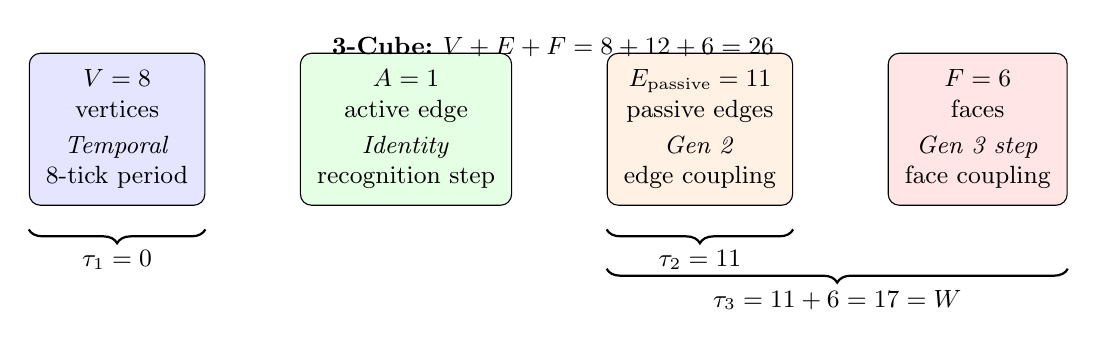
\begin{tikzpicture}[
  box/.style={draw, rounded corners, align=center, inner sep=6pt, font=\small,
              minimum width=22mm},
  >=Stealth
]
  \node[box, fill=blue!10] (V) {$V=8$\\vertices\\[2pt]\emph{Temporal}\\8-tick period};
  \node[box, fill=green!10, right=12mm of V] (A) {$A=1$\\active edge\\[2pt]\emph{Identity}\\recognition step};
  \node[box, fill=orange!10, right=12mm of A] (Ep) {$\Epass=11$\\passive edges\\[2pt]\emph{Gen~2}\\edge coupling};
  \node[box, fill=red!10, right=12mm of Ep] (F) {$F=6$\\faces\\[2pt]\emph{Gen~3 step}\\face coupling};

  \node[above=8mm of $(A)!0.5!(Ep)$, font=\small\bfseries] {3-Cube:\ $V+E+F=8+12+6=26$};

  \draw[decorate,decoration={brace,amplitude=5pt,mirror},thick]
    ([yshift=-3mm]V.south west) -- node[below=4pt,font=\small] {$\tau_1=0$} ([yshift=-3mm]V.south east);
  \draw[decorate,decoration={brace,amplitude=5pt,mirror},thick]
    ([yshift=-3mm]Ep.south west) -- node[below=4pt,font=\small] {$\tau_2=11$} ([yshift=-3mm]Ep.south east);
  \draw[decorate,decoration={brace,amplitude=5pt,mirror},thick]
    ([yshift=-8mm]Ep.south west) -- node[below=4pt,font=\small] {$\tau_3=11+6=17=W$} ([yshift=-8mm]F.south east);
\end{tikzpicture}
\caption{The full combinatorial partition of the 3-cube into physical roles.
Every element is assigned exactly once.  The generation torsion $\{0,11,17\}$
arises from the cumulative coupling to passive edges and faces.}
\label{fig:partition}
\end{figure}


%=============================================================================
\section{The Universality of Generation Torsion Across Sectors}
\label{sec:universality}
%=============================================================================

\subsection{Why the torsion is sector-independent}

The generation torsion $\{0,11,17\}$ is the same in every sector
(leptons, up quarks, down quarks).  This universality follows from the
derivation: the torsion values are cube combinatorial elements ($\Epass$
and $F$), which are properties of the cube itself, not of any particular
particle or charge.

What differs between sectors is:
\begin{itemize}[nosep]
  \item The \textbf{sector baseline} $\ell_{\mathrm{sector}}$
        (the rung of the lightest member): $\ell_e=2$, $\ell_u=4$, $\ell_d=4$.
  \item The \textbf{sector yardstick} $(B_{\mathrm{pow}},r_0)$
        (the overall scale).
  \item The \textbf{charge band} $Z$ (the gap function value).
\end{itemize}

But the \emph{generation spacing}---the rung difference between generations
within a sector---is universal: $+11$ for gen-1$\to$2, $+6$ for gen-2$\to$3,
in every sector.

\subsection{The Lean verification}

The universality is machine-verified in
\texttt{IndisputableMonolith.Masses.RungConstructor.Proofs}: the
\texttt{match\_rsbridge\_rung} theorem proves that
\texttt{compute\_rung(.fermion f) = RSBridge.rung f} for \emph{all}
fermion species $f$, confirming that the constructor (which uses the
universal torsion) reproduces the complete rung table.


%=============================================================================
\section{Falsifiers}
\label{sec:falsifiers}
%=============================================================================

\begin{enumerate}
  \item \textbf{Fourth generation discovery}.  If a fourth generation of
        fermions is discovered with SM-like gauge charges, the three-level
        combinatorial argument must be extended.  The framework predicts
        no fourth generation below the Planck scale.

  \item \textbf{Non-universal generation spacing}.  If the generation mass
        ratios in different sectors, when transported to $\muStar$, show
        qualitatively different exponent structures (e.g., the lepton
        gen-1$\to$2 step is~11 but the quark gen-1$\to$2 step is~9),
        the universality of cube-derived torsion is refuted.

  \item \textbf{Generation step ratio}.  The ratio $\Delta_{1\to 2}/\Delta_{2\to 3}=11/6$
        implies a specific, measurable asymmetry in the generation hierarchy.
        If precision measurements and RG transport establish a ratio
        inconsistent with $11/6$, the edge-face decomposition is refuted.

  \item \textbf{Alternative dimension}.  If any $D\neq 3$ is shown to produce
        a consistent RS framework with the same predictive power, the
        dimensional coincidence theorem loses its force.
\end{enumerate}


%=============================================================================
\section{Discussion}
\label{sec:discussion}
%=============================================================================

\subsection{Comparison with other generation models}

Various approaches to the generation problem exist in the literature:
\begin{itemize}[nosep]
  \item \textbf{Discrete flavor symmetries} ($A_4$, $S_4$, $\Delta(27)$, etc.)
        can produce three generations but require choosing the symmetry group
        as an input and introducing vacuum alignment sectors.
  \item \textbf{Extra dimensions} (Kaluza--Klein) can produce a tower of
        generations but require a specific compactification geometry.
  \item \textbf{Preon models} generate generations from composite structure
        but introduce new dynamics.
\end{itemize}

The RS approach is distinguished by having \emph{no choice}: the number of
generations is not selected by choosing a symmetry group or compactification
manifold.  It is forced by the combinatorial hierarchy of the 3-cube, which
is itself forced by $D=3$, which is itself forced by the linking and
gap-45 synchronization requirements.

\subsection{The deeper question: why is the cube sufficient?}

The remarkable fact is not just that the cube has three levels of spatial
structure, but that these three levels \emph{exactly exhaust} the cube's
combinatorial content when combined with the temporal structure.  The
partition $8+1+11+6=26$ leaves no room for additional physical roles.
This suggests that the 3-cube is not merely \emph{compatible} with the
observed particle content but is \emph{saturated} by it: nature uses
every piece of the cube's geometry exactly once.


%=============================================================================
\section{Conclusions}
\label{sec:conclusions}
%=============================================================================

This paper has derived the generation torsion $\{0,11,17\}$ from the
combinatorial hierarchy of the 3-cube, showing that:

\begin{enumerate}[nosep]
  \item Each generation corresponds to a level of geometric coupling:
        active edge only (gen~1), passive edges (gen~2), faces (gen~3).

  \item The generation steps are $\Delta_{1\to 2}=\Epass=11$ and
        $\Delta_{2\to 3}=F=6$, with cumulative torsion
        $\tau_3=\Epass+F=17=W$.

  \item The identity $\Epass(D)+F(D)=W$ holds if and only if $D=3$
        (Theorem~\ref{thm:coincidence}), linking the generation structure to
        three-dimensionality.

  \item Exactly three generations exist because the 3-cube has exactly
        three levels of spatial combinatorial structure.

  \item The cube's elements partition exhaustively into physical roles:
        $V=8$ (temporal), $A=1$ (active edge), $\Epass=11$ (gen-2 torsion),
        $F=6$ (gen-3 step), with $8+1+11+6=26=V+E+F$.

  \item The generation torsion is universal across sectors (leptons,
        up quarks, down quarks) because it derives from cube geometry,
        not from charge or sector properties.
\end{enumerate}

The generation puzzle---why three families, why these mass ratios,
why universal across sectors---is resolved by a single observation:
the 3-cube's combinatorial hierarchy has exactly three spatial levels,
and nature uses all of them.

\begin{thebibliography}{99}
\bibitem{PDG2024} R.~L.~Workman \textit{et al.} [Particle Data Group],
  Prog.\ Theor.\ Exp.\ Phys.\ \textbf{2022}, 083C01 (2022) and 2024 update.
\bibitem{Fedorov1891} E.~S.~Fedorov,
  ``Simmetriya pravil'nykh sistem figur''
  [Symmetry of regular systems of figures],
  Zapiski Imp.\ S.-Peterburgskogo Mineral.\ Obshch.\ \textbf{28}, 1--146 (1891).
\bibitem{Polya1924} G.~P\'olya,
  ``\"Uber die Analogie der Kristallsymmetrie in der Ebene,''
  Z.~Kristallogr.\ \textbf{60}, 278--282 (1924).
\bibitem{Washburn2025} J.~Washburn,
  ``The Algebra of Reality: A Recognition Science Derivation of Physical Law,''
  \textit{Axioms} \textbf{15}(2), 90 (2025).
\bibitem{PaperI} J.~Washburn, Paper~I of this series.
\bibitem{PaperII} J.~Washburn, Paper~II of this series.
\bibitem{PaperV} J.~Washburn, Paper~V of this series.
\end{thebibliography}

\end{document}
